\documentclass[10pt]{beamer}

\usetheme{CambridgeUS}
\usepackage[english, russian]{babel}
\usepackage[utf8]{inputenc}
\usepackage{caption}
\usepackage{etoolbox}
\usepackage{multicol}
\usepackage{listings}
\usepackage{wasysym}
\usepackage{mathtools}
\DeclarePairedDelimiter\ceil{\lceil}{\rceil}
\DeclarePairedDelimiter\floor{\lfloor}{\rfloor}

\definecolor{mygreen}{rgb}{0,0.6,0}
\lstset{
  basicstyle=\ttfamily\footnotesize,        % the size of the fonts that are used for the code
  breaklines=true,                 % automatic line breaking only at whitespace
  captionpos=b,                    % sets the caption-position to bottom
  commentstyle=\color{mygreen},    % comment style
  keywordstyle=\color{blue},       % keyword style
  stringstyle=\color{red},     % string literal style
  showstringspaces=false,
  morekeywords={include, printf},
  texcl=true     %<---- added
}


\title[\href{https://goo.gl/NRgp8K}{https://goo.gl/NRgp8K} (Term 1)]{A-Star. Пятнашки}
\author[Гусев Илья, Булгаков Илья]{Гусев Илья, Булгаков Илья}
\institute[МФТИ] 
{Московский физико-технический институт\\*}
\date{Москва, 2019}
\subject{Computer Science}

\begin{document}

\begin{frame}
  \titlepage
\end{frame}

\begin{frame}{Содержание}
\tableofcontents
\end{frame}

\section{Правила игр Пятнашки и Восьминашки}

\begin{frame}[fragile]{Игра Пятнашки}
\begin{center}
    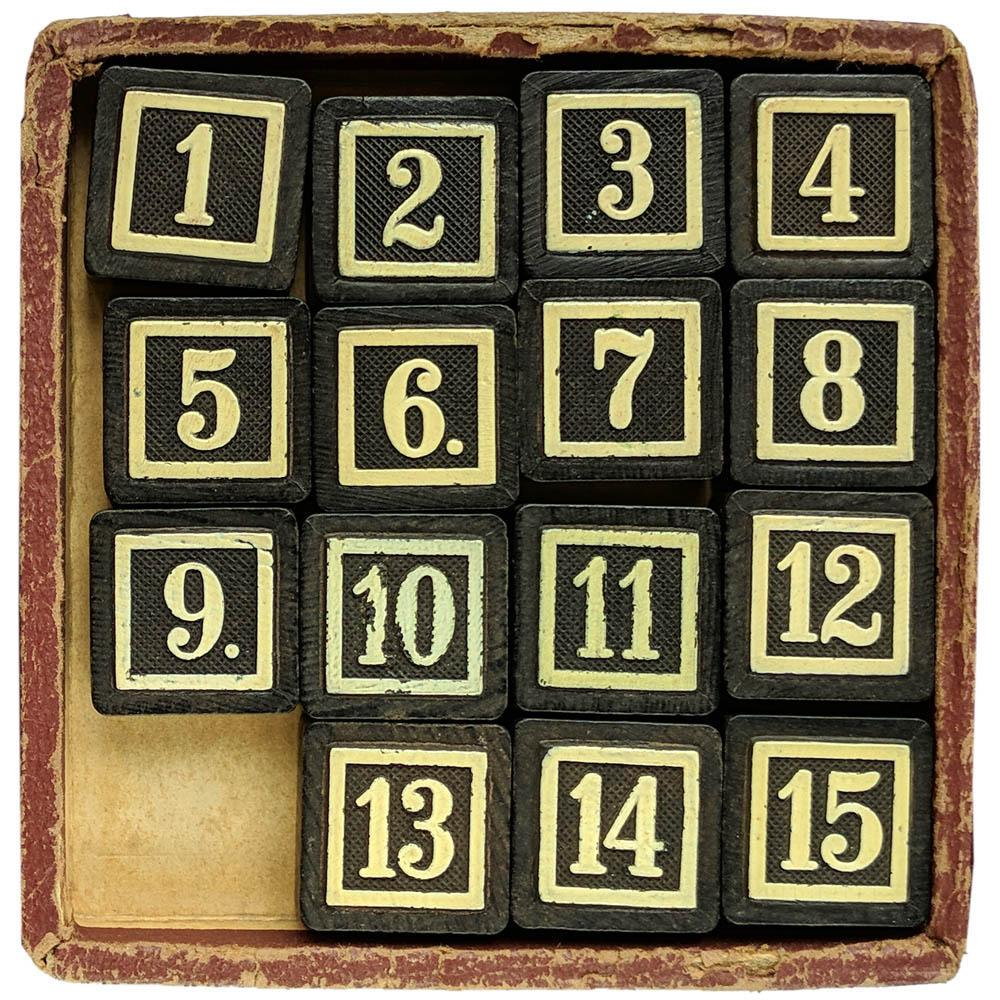
\includegraphics[width=7cm]{Term_2/Source/images/15puzzle.jpg}
\end{center}
\end{frame}

\begin{frame}[fragile]{Правила игры Пятнашки}

\begin{center}
    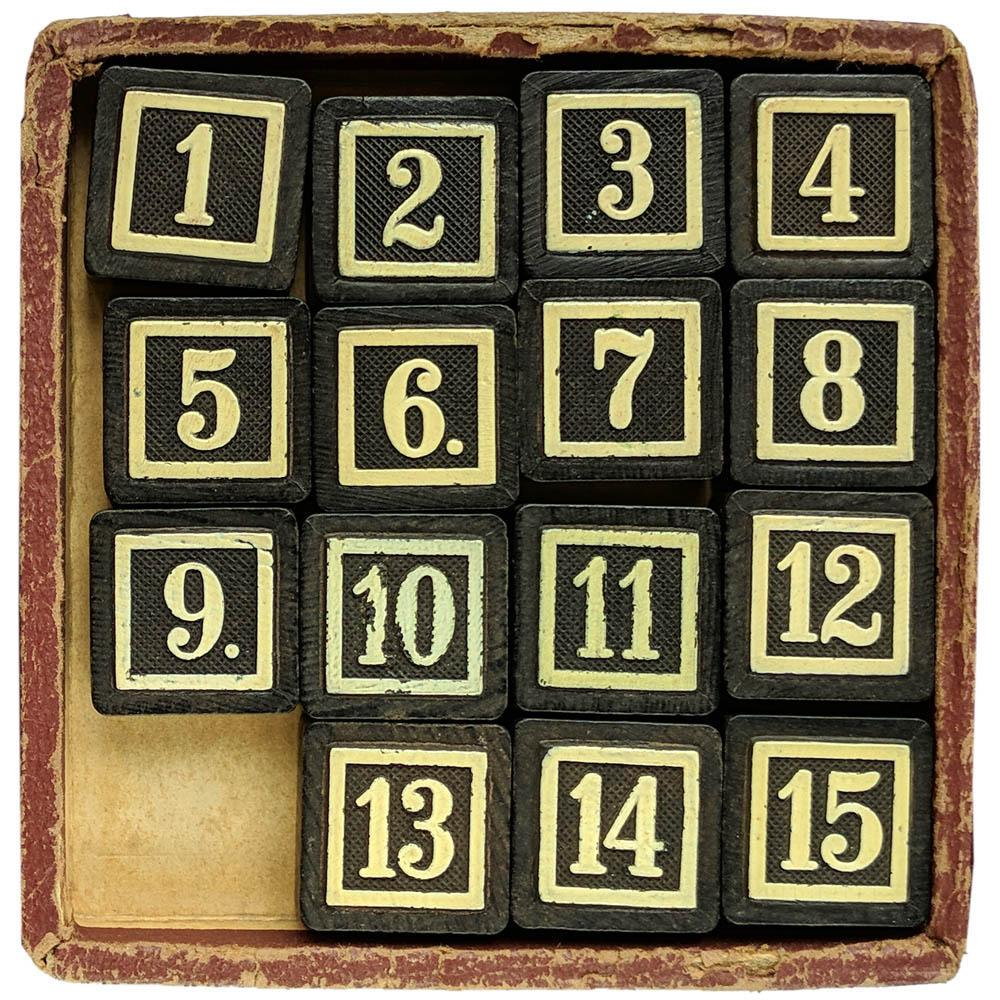
\includegraphics[width=3cm]{Term_2/Source/images/15puzzle.jpg}
\end{center}

\begin{itemize}
    \item 15 карточек с числами от 1 до 15
    \item Одно пустое поле
    \item Доступна операция сдвига карточки с числом на соседнее поле, если оно пусто
    \item Цель игры — перемещая костяшки по коробке, добиться упорядочивания их по номерам, желательно сделав как можно меньше перемещений.
\end{itemize}

\end{frame}

\begin{frame}[fragile]{Правила игры Восьминашки}
\begin{center}
    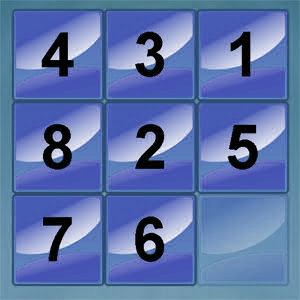
\includegraphics[width=3cm]{Term_2/Source/images/8puzzle.png}
\end{center}
\begin{itemize}
    \item 8 карточек с числами от 1 до 8
    \item Одно пустое поле
    \item Доступна операция сдвига карточки с числом на соседнее поле, если оно пусто
    \item Цель игры — перемещая костяшки по коробке, добиться упорядочивания их по номерам, желательно сделав как можно меньше перемещений.
\end{itemize}
\end{frame}

\section{Разбор игры Восьминашки}

\begin{frame}[fragile]{Игра Восьминашки}
Любую ли перестановку можно получить из другой?
\begin{center}
    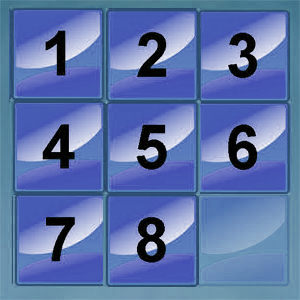
\includegraphics[width=3cm]{Term_2/Source/images/8puzzle_correct_even.png} 
    \\
    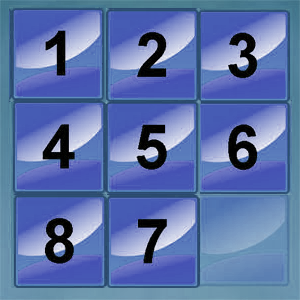
\includegraphics[width=3cm]{Term_2/Source/images/8puzzle_odd.png}
\end{center}
\end{frame}

\begin{frame}[fragile]{Игра Восьминашки}
\begin{itemize}
    \item Перестановка множества  S  содержит инверсию элементов  $i_j$  и  $i_k$ , если нарушен их естественный порядок расположения, т.е. больший элемент расположен левее меньшего: $i_j$ >  $i_k$  при $(j < k)$.
    \item Считаем число инверсий в перестановке \\
    12345678 - 0 инверсий \\
    12345687 - 1 инверсия
    \item Меняет ли ход в игре восьминашки четность перестановки?
\end{itemize}
\begin{center}
    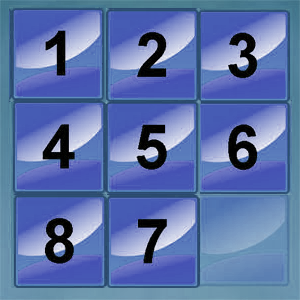
\includegraphics[width=3cm]{Term_2/Source/images/8puzzle_odd.png}
\end{center}
\end{frame}


\begin{frame}[fragile]{Игра Восьминашки}
Как будем искать решение задачи? Помогут графы!
\begin{itemize}
    \item Состояние доски - вершина. Ход - ребро.
    \item Нужно найти путь из одной вершины в другую.
    \item Какие есть алгоритмы? Взвешенный у нас граф или нет?
\end{itemize}
\begin{center}
    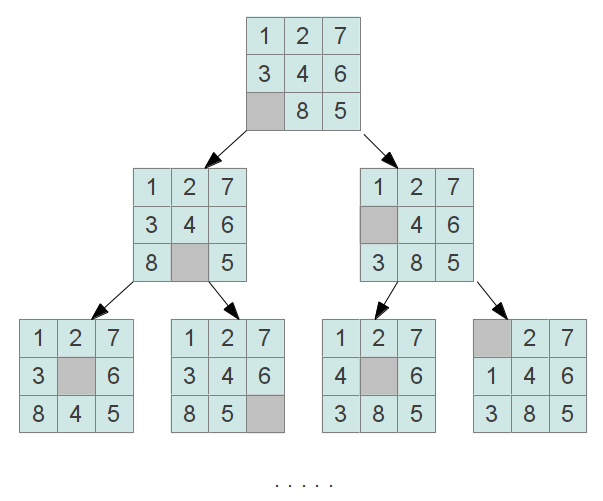
\includegraphics[width=6cm]{Term_2/Source/images/8_perebor.png}
\end{center}
\end{frame}

\begin{frame}[fragile]{Игра Восьминашки}
Почему поиск в ширину работает?
\begin{itemize}
    \item Сколько у нас перестановок? $8! / 2$ =  ок. 180000. Обойти реально.
    \item Как будем представлять одно состояние доски? Какую структуру использовать?
\end{itemize}
\begin{center}
    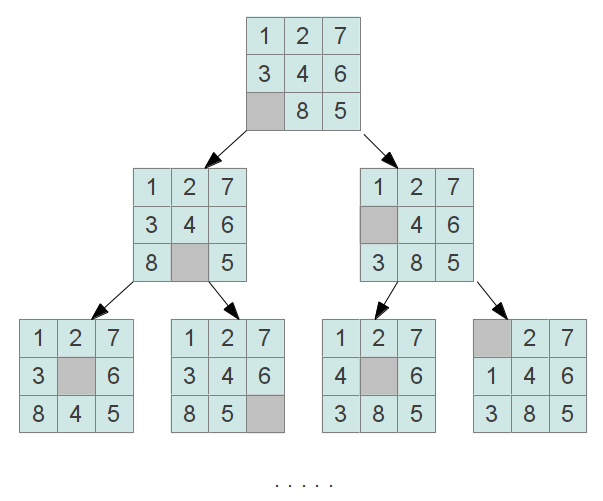
\includegraphics[width=6cm]{Term_2/Source/images/8_perebor.png}
\end{center}
\end{frame}

\section{Разбор игры Пятнашки}

\begin{frame}[fragile]{Игра Пятнашки}
Как будем решать? Надо ли что-то менять по сравнению с восьминашками?
\begin{center}
    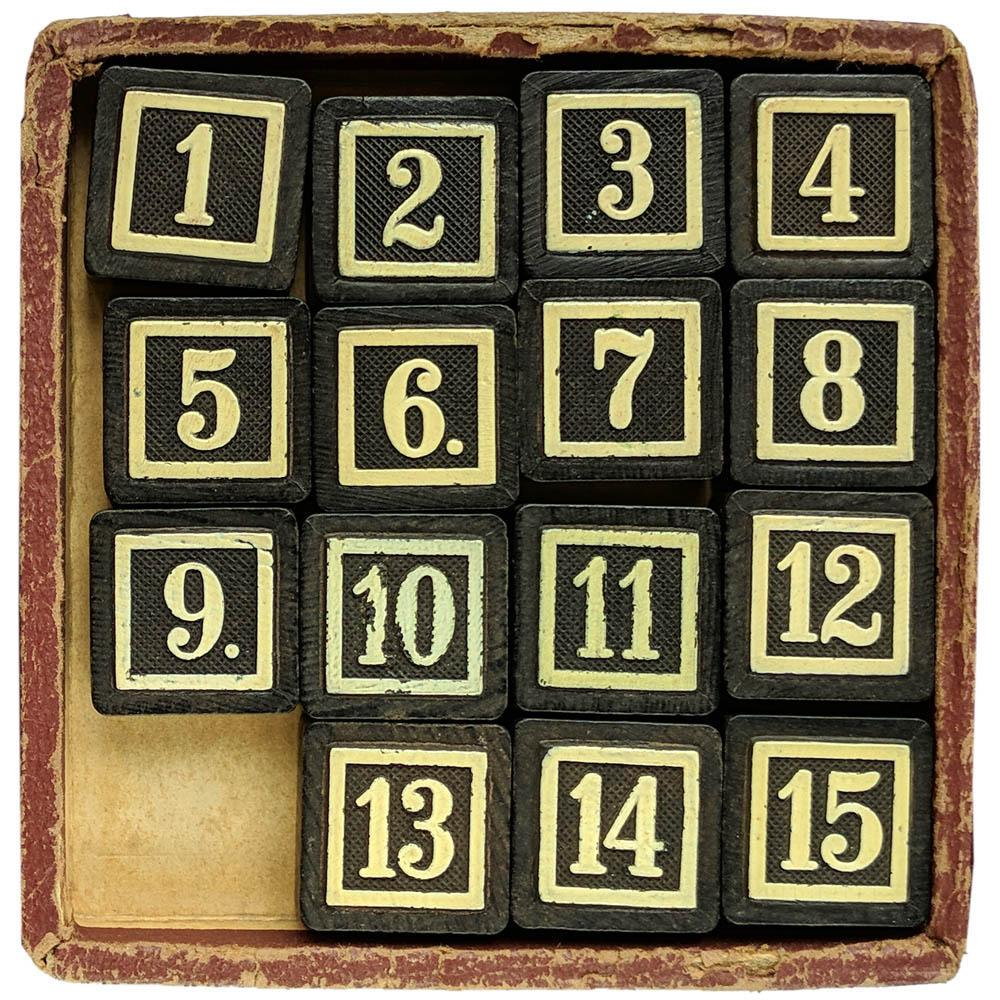
\includegraphics[width=6cm]{Term_2/Source/images/15puzzle.jpg}
\end{center}
\end{frame}

\begin{frame}[fragile]{Игра Пятнашки}
\begin{itemize}
    \item Меняется условие на достижимость одной перестановки из другой.
    \item Как будем представлять одно состояние доски? Какую структуру использовать?
    \item Обход в ширину не поможет $15! / 2$ = ок. 600 млрд. Обойти нереально.
\end{itemize}
\begin{center}
    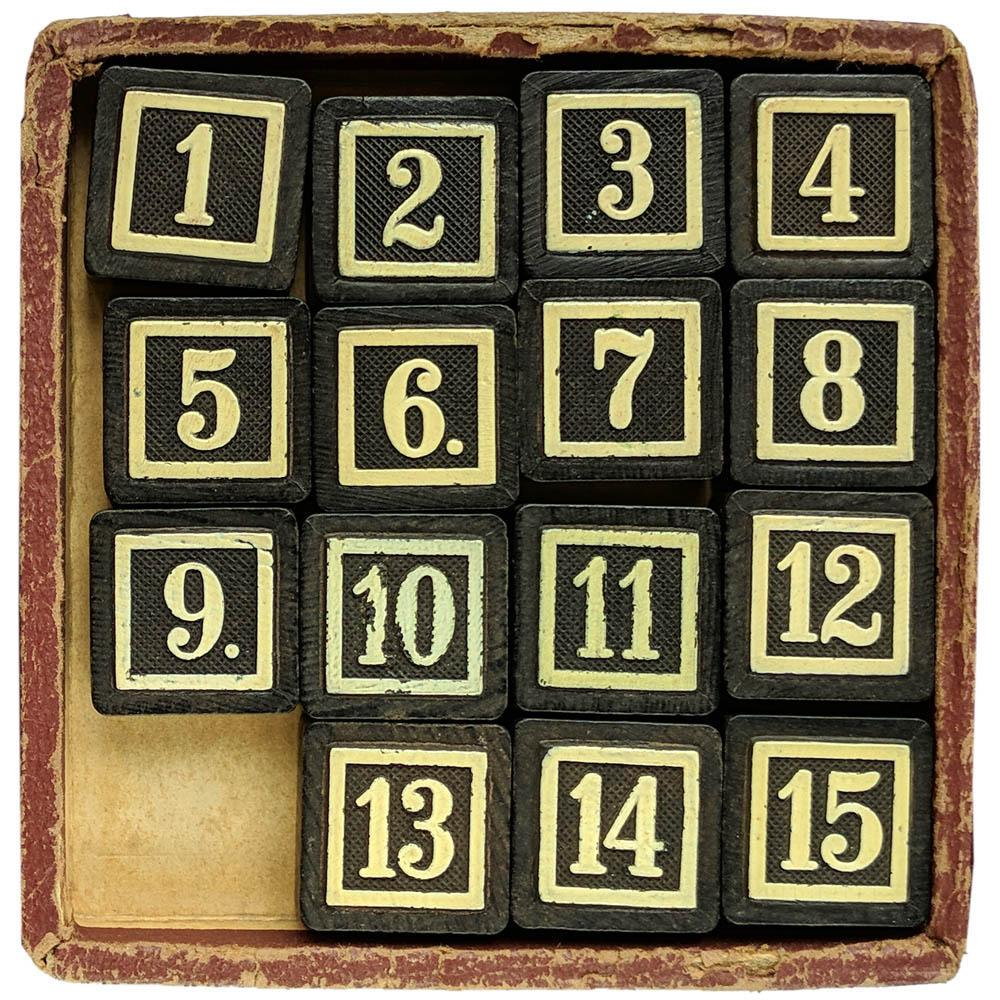
\includegraphics[width=4cm]{Term_2/Source/images/15puzzle.jpg}
\end{center}
\end{frame}

\begin{frame}[fragile]{Игра Пятнашки}
\begin{itemize}
    \item Условие на достижимость: четность перестановки без 0 + номер строки, где находится 0. 
    \item Представление состояния: плотная упаковка. 64-битное целое, на каждую ячейку по 4 бита.
    \item Вместо обхода в ширину -- \textbf{другой алгоритм}, более умный!
\end{itemize}
\begin{center}
    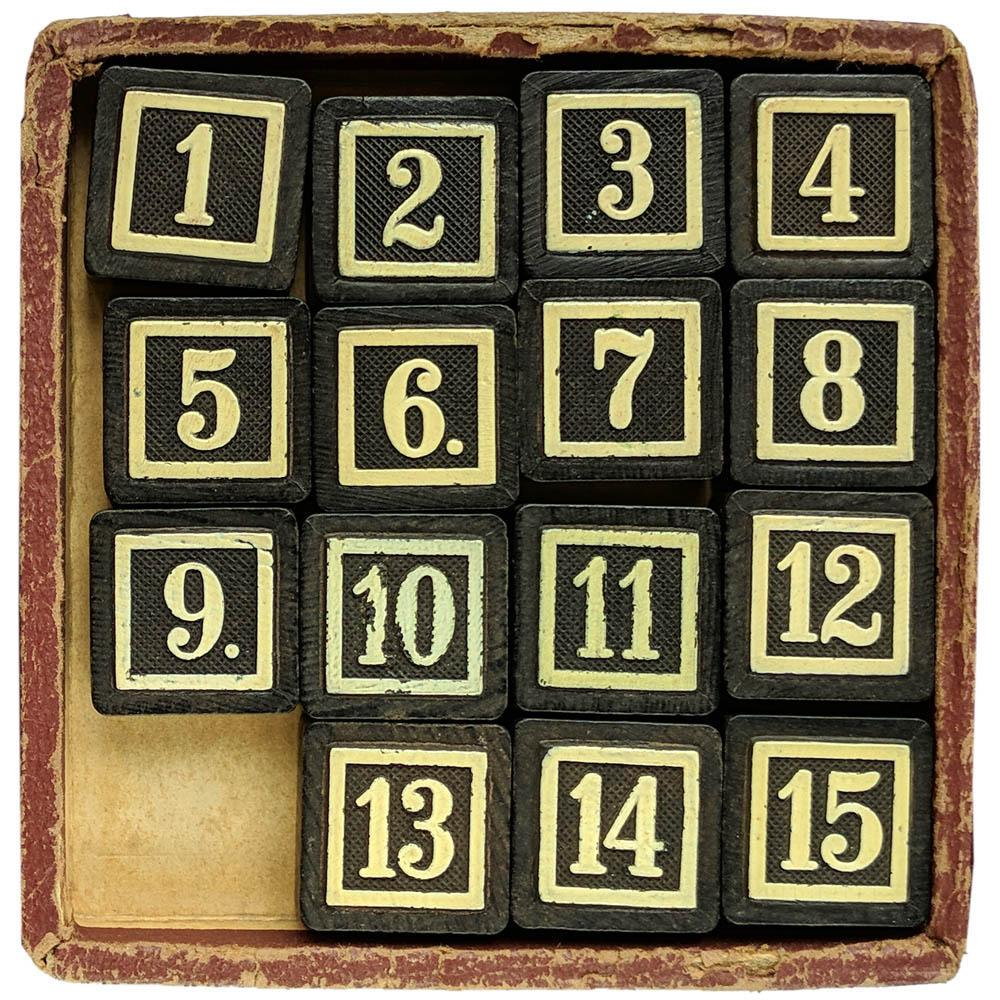
\includegraphics[width=4cm]{Term_2/Source/images/15puzzle.jpg}
\end{center}
\end{frame}

\section{Алгоритм A*}

\begin{frame}[fragile]{Вспоминаем: алгоритм Дейкстры}
\begin{center}
    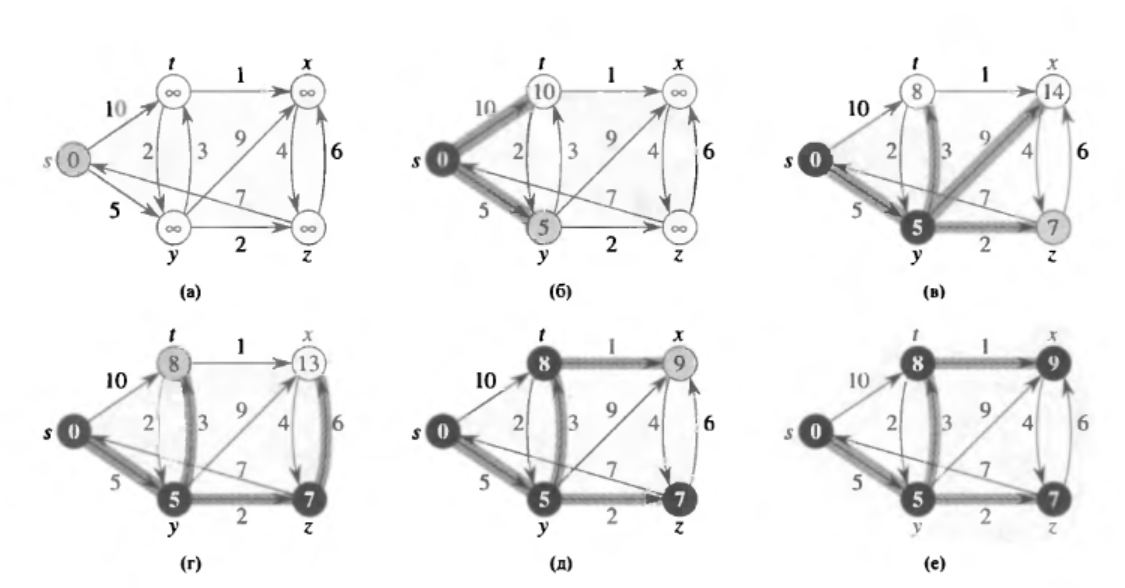
\includegraphics[width=12cm]{Term_2/Source/images/dijkstra.png}
\end{center}
\end{frame}

\begin{frame}[fragile]{Вспоминаем: алгоритм Дейкстры}
\begin{center}
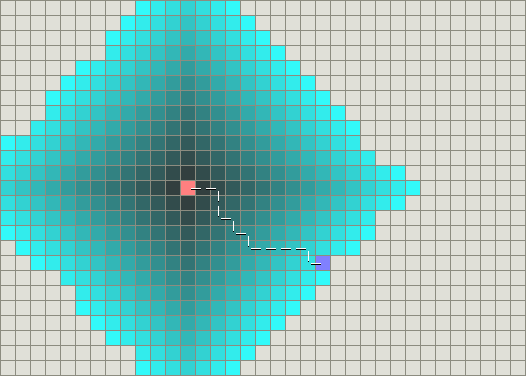
\includegraphics[width=9cm]{Term_2/Source/images/dijkstra-new.png}
\end{center}
\end{frame}

\begin{frame}[fragile]{Эвристика}
Эвристика — оценка расстояние от вершины до целевой вершины.\\
Мы берём эвристику, исходя из знаний о среде
\end{frame}

\begin{frame}[fragile]{Эвристика: примеры}
Среда: квадратная сетка с 4 направлениями движения\\
Эвристика: манхэттенское расстояние
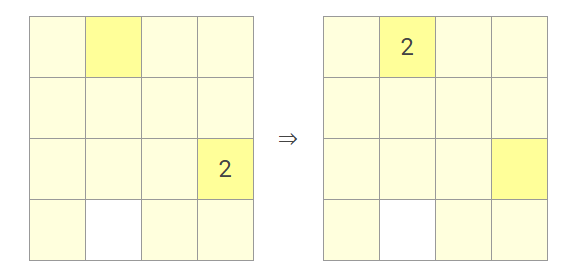
\includegraphics[width=12cm]{Term_2/Source/images/manhattan.png}
\end{frame}

\begin{frame}[fragile]{Эвристика: примеры}
Среда: произвольная карта\\
Эвристика: евклидово расстояние
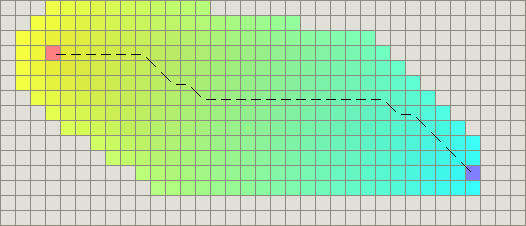
\includegraphics[width=10cm]{Term_2/Source/images/euclidean.png}
\end{frame}

\begin{frame}[fragile]{Greedy Best-First-Search}
Минимизация расстояния от S $\Rightarrow$ маскимизация эвристики до T
\begin{center}
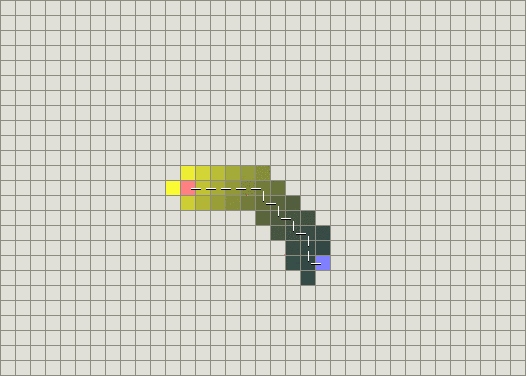
\includegraphics[width=9cm]{Term_2/Source/images/best-first-search.png}
\end{center}
\end{frame}

\begin{frame}[fragile]{Препятствия (Дейкстра)}
\begin{center}
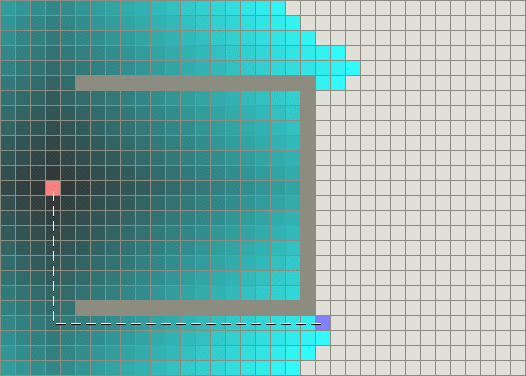
\includegraphics[width=9cm]{Term_2/Source/images/dijkstra-trap.png}
\end{center}
\end{frame}

\begin{frame}[fragile]{Препятствия (GBFS)}
\begin{center}
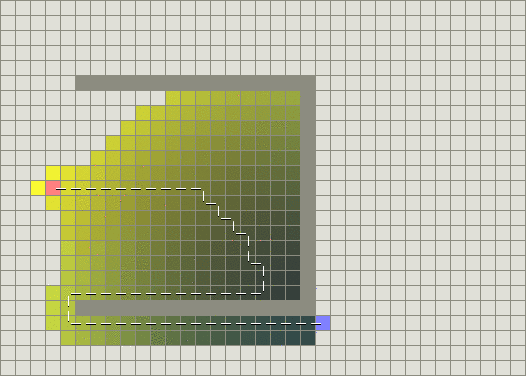
\includegraphics[width=9cm]{Term_2/Source/images/best-first-search-trap.png}
\end{center}
\end{frame}

\begin{frame}[fragile]{A*}
A* = Дейкстра + эвристика\\
$f(n) = g(n) + h(n)$, где \\
g(n) - минимальное расстояние от стартовой точки (вершины)\\
h(n) - эвристическое расстояние до конечной точки (вершины)\\
f(n) - итоговая оценка точки (вершины) \\
\end{frame}

\begin{frame}[fragile]{Препятствия (A*)}
\begin{center}
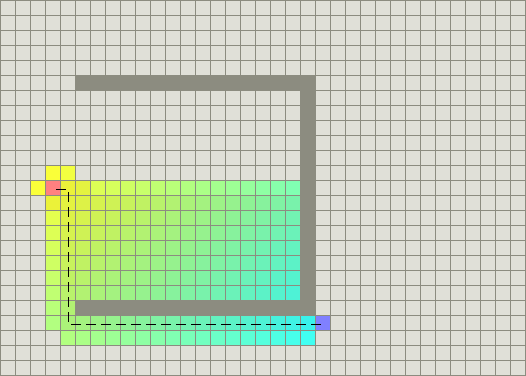
\includegraphics[width=9cm]{Term_2/Source/images/a-star-trap.png}
\end{center}
\end{frame}

\begin{frame}[fragile]{Свойства эвристики}
\begin{enumerate}
    \item $\forall n, h(n) = 0 \Rightarrow$ обычный Дейкстра с гарантией кратчайшего пути
    \item Допустимость: $\forall n, h(n) \leq f(n, T) \Rightarrow$ A* с гарантией кратчайшего пути
    \item Чем меньше h(n), тем больше вершин обходится
    \item Монотонность: $\forall n, p: \exists E(n, p) \rightarrow h(n)-h(p) \leq w(n, p)$, $h(T) = 0$
    \item Монотонность $\Rightarrow$ допустимость
    \item $\forall n, h(n) = f(n, T) \Rightarrow$ всегда идеальный путь
    \item h(n) может переоценивать f(n, T), но тогда путь может быть неоптимальным
\end{enumerate}
\end{frame}

\section{Эвристики для Пятнашек}

\begin{frame}[fragile]{Эвристики для Пятнашек}
\begin{enumerate}
    \item Манхэттенское расстояние
    \item Линейный конфликт
    \item Угловые фишки
    \item Последний ход
\end{enumerate}
\end{frame}

\begin{frame}[fragile]{Эвристики для Пятнашек}
\textbf{Манхэттенское расстояние} -- это сумма расстояний по строкам и столбцам от текущего расположения костяшки до ее правильной позиции \\
На примере ниже манхэттенское расстояние -- 4.
\begin{center}
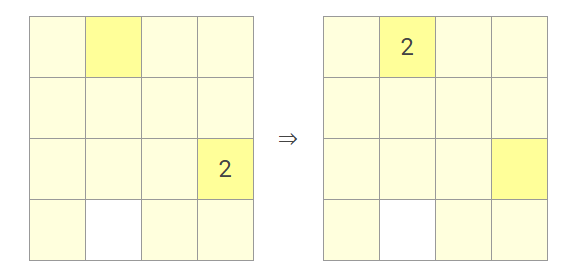
\includegraphics[width=8cm]{Term_2/Source/images/manhattan_15.png}
\end{center}
\end{frame}

\begin{frame}[fragile]{Эвристики для Пятнашек}
Считается, что костяшка I и костяшка J находятся в \textbf{линейном конфликте} по строке, если они обе стоят в своей строке, но костяшка I находится левее костяшки J, хотя на самом деле должна быть справа. \\
На этой схеме I = 15, J = 13.
\\
Мы должны подвинуть одну из костяшек со строки, поэтому можем добавить 2 к манхэттенскому расстоянию. Аналогичным образом рассматривается линейный конфликт по столбцу.
\begin{center}
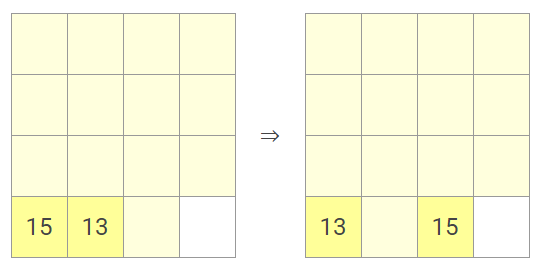
\includegraphics[width=8cm]{Term_2/Source/images/linear_conflict.png}
\end{center}
\end{frame}



\begin{frame}[fragile]{Эвристики для Пятнашек}
\textbf{Угловые фишки}. Рассмотрим правый верхний угол. Пусть «3» или «8» стоит на своей позиции, а на месте «4» — любая другая костяшка
\\
В таком случае, чтобы поставить «4» на место, костяшки придется подвинуть. Для этого добавим 2 к манхэттенскому расстоянию. Если «3» или «8» участвует в линейном конфликте (linear conflict), то двойка уже добавлена.
\\
Аналогично с левым верхним и левым нижним углами. Правый нижний угол в эвристике не рассматривается, так как очень сложно скомбинировать этот случай с эвристикой «Последний ход».
\begin{center}
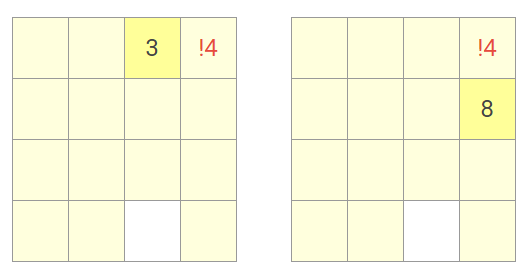
\includegraphics[width=6cm]{Term_2/Source/images/corner.png}
\end{center}
\end{frame}

\begin{frame}[fragile]{Эвристики для Пятнашек}
\textbf{Последний ход.} На последнем ходу мы либо двигаем костяшку «15» влево, либо «12» — вверх
\\
Если костяшки не находятся на требуемых позициях («15» — в крайнем правом ряду или «12» — в самой нижней строке), манхэттенское расстояние не учитывает переход через угол. Поэтому мы можем добавить к нему 2.
\begin{center}
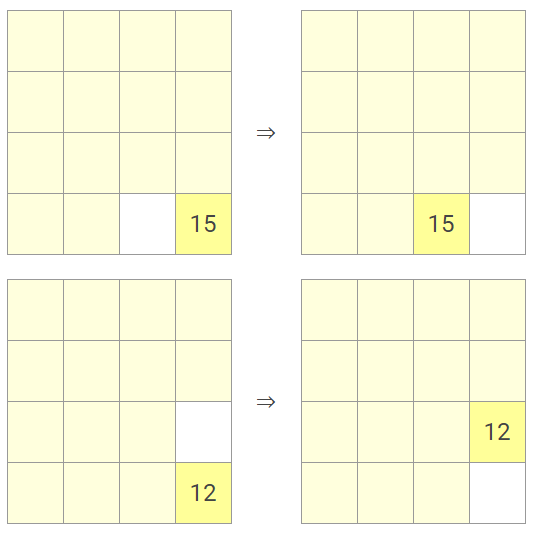
\includegraphics[width=4cm]{Term_2/Source/images/last_move.png}
\end{center}
\end{frame}




\appendix

\begin{frame}[allowframebreaks]
  \frametitle<presentation>{Полезные ссылки}
    
  \begin{thebibliography}{10}
{
  \beamertemplatebookbibitems
  % Start with overview books.
    
\bibitem{stanford}
  \texttt{Amit’s A* Pages From Red Blob Games}
  \newblock \href{http://theory.stanford.edu/~amitp/GameProgramming/}{\texttt{http://theory.stanford.edu/~amitp/GameProgramming/}}

  \bibitem{neercwiki}
  \texttt{neerc.ifmo.ru: Алгоритм A*}
  \newblock \href{https://bit.ly/2q3RbJg}{\texttt{https://bit.ly/2q3RbJg}}
  
  \bibitem{wiki1}
  \texttt{Wiki: A* search algorithm}
  \newblock \href{https://en.wikipedia.org/wiki/A*_search_algorithm}{\texttt{https://en.wikipedia.org/wiki/A*\_search\_algorithm}}
  
   \bibitem{wiki2}
  \texttt{Wiki: admissible heuristic}
  \newblock \href{https://en.wikipedia.org/wiki/Admissible_heuristic}{\texttt{https://en.wikipedia.org/wiki/Admissible\_heuristic}}
  
  
  
}
    
  \end{thebibliography}
\end{frame}

\end{document}


